\documentclass[tikz,border=8pt]{standalone}
\usetikzlibrary{arrows.meta,positioning}
\begin{document}
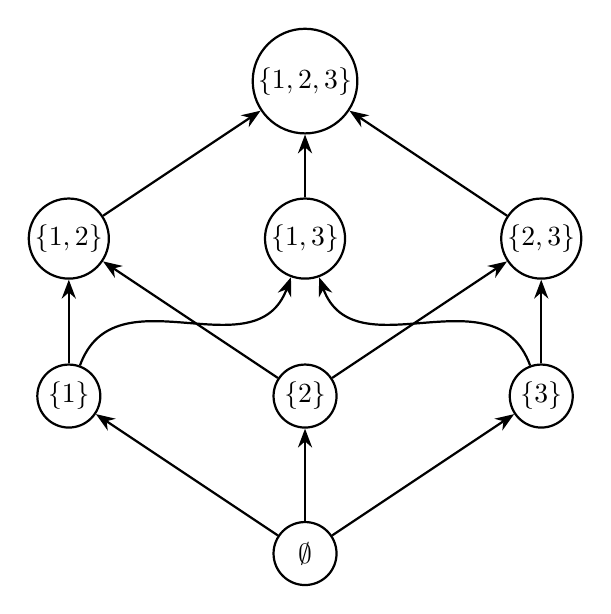
\begin{tikzpicture}[x=1cm,y=1cm]
\tikzset{
  graphnode/.style={circle,draw,thick,minimum size=8mm,inner sep=1pt,font=\sffamily},
  directed/.style={-{Stealth[length=2.4mm]},thick},
  undirected/.style={thick}
}
\node[graphnode] (n_E) at (0.00,0.00) {$\emptyset$};
\node[graphnode] (n_S1) at (-3.00,2.00) {$\{1\}$};
\node[graphnode] (n_S2) at (0.00,2.00) {$\{2\}$};
\node[graphnode] (n_S3) at (3.00,2.00) {$\{3\}$};
\node[graphnode] (n_P12) at (-3.00,4.00) {$\{1,2\}$};
\node[graphnode] (n_P13) at (0.00,4.00) {$\{1,3\}$};
\node[graphnode] (n_P23) at (3.00,4.00) {$\{2,3\}$};
\node[graphnode] (n_F) at (0.00,6.00) {$\{1,2,3\}$};
\draw[directed] (n_E) -- (n_S1);
\draw[directed] (n_E) -- (n_S2);
\draw[directed] (n_E) -- (n_S3);
\draw[directed] (n_S1) -- (n_P12);
\draw[directed] (n_S1) to[out=70,in=250,looseness=1.15] (n_P13);
\draw[directed] (n_S2) -- (n_P12);
\draw[directed] (n_S2) -- (n_P23);
\draw[directed] (n_S3) to[out=110,in=290,looseness=1.15] (n_P13);
\draw[directed] (n_S3) -- (n_P23);
\draw[directed] (n_P12) -- (n_F);
\draw[directed] (n_P13) -- (n_F);
\draw[directed] (n_P23) -- (n_F);
\end{tikzpicture}
\end{document}
